In this chapter, we formulate the design goals that our implementation should meet
and then discuss four possible implementation approaches.

\section{Design goals}\label{sec:design-goals}
After analyzing the KeePass plugin system and FIDO2 capabilities, we can now formulate how the combination of KeePass
and a FIDO2 authenticator could look in more detail:

\begin{enumerate}
	\item Websites that support FIDO2 can use this form of authentication exclusively, without passwords.
	\item For websites that do not support FIDO2, a regular password stored in KeePass can be used.
	\begin{enumerate}
		\item For websites that support the older U2F, the FIDO2 device can be used for additional security as a second factor.
		\item The KeePass database can be unlocked by the FIDO2 device instead of a master password.
	\end{enumerate}
\end{enumerate}

Our implementation will, therefore, be a KeePass key provider plugin to make the point 2b possible.

An important fact to keep in mind is that KeePass does not support keys being used alternatively,
i.e., when a database is configured to be protected by a master password and a custom key provider,
they are \emph{both} required to unlock it. It is not possible to configure it, at least by the end-user, in such a way
that the unlock methods could be used interchangeably~\cite{keepass:keys}.

This is not ideal because introducing a custom key provider means the database cannot be unlocked
on other clients unless they also implement the same key provider, and one of our goals was preserving
database compatibility with other clients.

There are, however, ways to bypass this restriction. The QuickUnlock plugin introduced earlier does precisely
that\textemdash first, the database is unlocked using the full master key, and after that, only by a few of its characters.

When we examine its implementation closely, we can find that~\cite{keepass:plugin:quick-unlock}:

\begin{enumerate}
	\item When a database is created, the QuickUnlock plugin is \emph{not} registered as a key provider. Instead, the user uses a regular master password or a key file.
	\item Once the database is unlocked, the QuickUnlock plugin reads the database encryption key, which is available via the provided plugin interface, and stores this key in an encrypted form.
	\item The next time user is unlocking the database, they select the QuickUnlock provider. The QuickUnlock provider decrypts the previously stored master key using the short password entered by the user and unlocks the database with this master key.
\end{enumerate}

This approach means that while from the user's point of view, the database is being unlocked by the QuickUnlock plugin,
the used key is identical with the one KeyPass would derive from the master password, which means the QuickUnlock and
master password unlock method may be used interchangeably.

We can use a similar approach:

\begin{enumerate}
	\item When creating a database, the user chooses the primary key\textemdash a master password, a key file, or even another method implemented by another plugin.
	\item After the database is created, the user will have an option to associate a FIDO2 authenticator with it. In this step, our plugin will retrieve the encryption master key and store it in a secure way.
	\item During the next unlock, the user may choose our provider, and the master key will be retrieved and used.
\end{enumerate}

This approach means:

\begin{itemize}
	\item The user can always decide whether they want to use the primary unlock method or our plugin.
	\item Multiple authenticators may be associated with one database.
	\item If only one authenticator is associated and it gets lost, the primary method works as a backup.
\end{itemize}

Someone might object that one of our goals was to remove the usage of a master password,
and this approach still requires it. It is, however, important to note that if
the database is only used on systems where our plugin is available, the master password
is never needed. In theory, users who do not want to have anything to remember, can
create a database with a long and random password (which can be generated using the KeePass generator),
associate an authenticator with it right after, and then they do not need to remember the password.
The downside is that there is no backup unlock method in case they lose the authenticator, so this
would only be advisable if at least two authenticators are associated with the database.

\section{Implementation options}\label{sec:implementation-options}

We have established that we want to take the existing master key,
and store it, while "protecting" it by the authenticator. Now is the time to look at the technical possibilities of doing do.

\subsection{Key stored as an authenticator resident key}\label{subsec:key-stored-on-the-authenticator-as-a-resident-key}

The authenticator was designed to securely store private keys, so of course, the first idea might be:
can we take an existing key\textemdash the one generated by KeePass\textemdash and transfer it to the authenticator?

The answer is no, unfortunately, as the authenticator was designed to handle the whole process\textemdash including generating the credentials\textemdash
on its own, and there is no interface that would allow storing externally generated credentials~\cite{fido:ctap}.

\subsection{Key encrypted by the authenticator}\label{subsec:key-enrypted-by-the-authenticator}

Since we need to generate a new key pair on the authenticator, maybe we could use the private key from that pair
to encrypt the database master key, and then store the encrypted master key in the unencrypted section of the database header section~\cite{keepass:kdbx}.

This design, where an asymmetric key is only used to encrypt a symmetric key, and the symmetric key is then used to encrypt and decrypt the data,
can be found, for example, in \gls{OpenPGP}\footnote{\Glsdesc{OpenPGP}.} as seen in \autoref{fig:openpgp-message-encryption}~\cite{rfc4880}.

\begin{figure}[H]
	\centering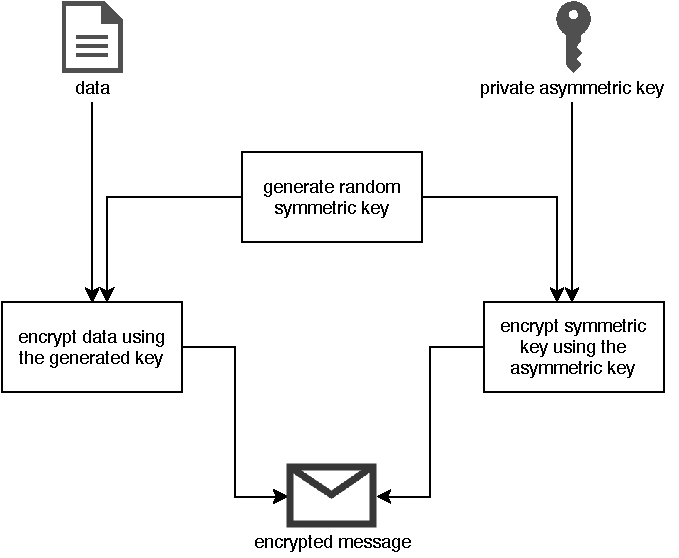
\includegraphics[width=\textwidth]{images/pgp}
	\caption{OpenPGP message encryption}
	\label{fig:openpgp-message-encryption}
\end{figure}

However, after inspecting the \glsxtrshort{ctap} specification, we find\textemdash similarly to the previous case\textemdash that while the authenticators
are likely technically capable of encrypting data\footnote{
	Considering that signing data typically involves the same underlying operations as encrypting it,
	and that authenticators may utilize encryption as a way to implement unlimited storage for non-resident credentials, as described in \autoref{subsec:webauthn}.
}, it is not something they were designed to do, so this functionality is not exposed
over their \glsxtrshort{api}~\cite{fido:ctap}.

\subsection{Encryption key derived from a signature}\label{subsec:encryption-key-derived-from-a-signature}

Following the previous ideas, we know that:

\begin{itemize}
	\item we cannot store the master key as a credential directly on the authenticator,
	\item we cannot use the authenticator directly to encrypt the key and store it elsewhere.
\end{itemize}

Given these constraints, let us take a close look at the one operation the authenticators support\textemdash signing data.
The \glsxtrshort{webauthn} specification does not specify the exact algorithm to be used. The authenticator
may implement any number of algorithms from the IANA \glsxtrfull{cose} Algorithms Registry~\cite{iana:cose-algorithms} and pick
one based on preferences expressed by the \gls{rp}~\cite{fido:webautn}. Generally, though, the commonly used signature schemes:

\begin{enumerate}
	\item take input data to be signed and a private key,
	\item apply some cryptographic operations on these two (the operations depend on the exact algorithm being used),
	\item output a "signature"~\cite{rfc8017}.
\end{enumerate}

\begin{figure}[H]
	\centering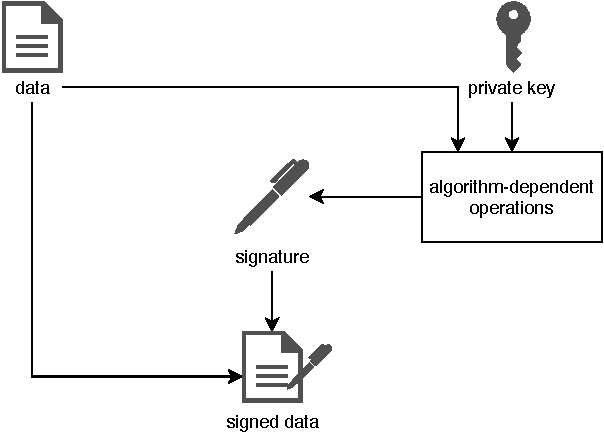
\includegraphics[width=\textwidth]{images/signature}
	\caption{A signature scheme with appendix}
	\label{fig:a-signature-scheme-with-appendix}
\end{figure}

The signature can be characterized by a few essential properties:

\begin{itemize}
	\item a user can efficiently produce their own signature on documents of their choice,
	\item other users can efficiently verify whether a given string is a signature of another (specific) user on a specific document,
	\item it is infeasible to produce signatures of other users to documents that they did not sign~\cite{the-foundations-of-cryptograpgy:vol-2}.
\end{itemize}

Usually, the purpose of a signature is to prove the authenticity of the signed data, i.e., the signature is considered
"public", but the fact that it is based on the private key, and cannot be created without its knowledge begs the question:
could the signature itself act as a key in an encryption scheme?

If yes, we might be able to do the following:

\begin{enumerate}
	\item Generate a resident credential on the authenticator.
	\item Generate random data to be signed (challenge) and store it in the database header section.
	\item Ask the authenticator to sign the challenge using the generated private key.
	\item Encrypt the database master key using the signature as an encryption key.
	\item Store the encrypted database master key in the database header section.
\end{enumerate}

To unlock the database without the master password, we would then:

\begin{enumerate}
	\item Take the stored challenge from the database header section.
	\item Ask the authenticator to sign it.
	\item Use the signature to decrypt the encrypted master key from the database header section.
	\item Use the database master key to unlock the database.
\end{enumerate}

Of course, this is not a typical usage of cryptographic primitives, so it brings several questions.

First, we need to make sure that repeatedly performing the sign operation using the same challenge and the same
credential always generates the same signature, since we use the signature for decryption. If it changed,
we would not be able to decrypt the master key. This is something that is not guaranteed, as it depends on
the chosen signature algorithm. We can, however, make a list of algorithms that have this property and
request that one them is used (and accept that the plugin will work only if the authenticator implements at least one such algorithm).

Note that the \glsxtrshort{webauthn} specification says that the challenges must be randomly generated by relying parties
to prevent replay attacks\footnote{A form of attack in which a valid data transmission is repeated by an adversary who intercepts and re-transmits it.}.
This requirement is based on the intended use-case\textemdash authentication\textemdash but is in direct contradiction with the
properties needed for encryption, as explained in the previous paragraph.

The second question is security. We know we will treat the signature itself as something "private",
and not store it anywhere. We also know it is created based on a private key stored on the authenticator
(which we assume to be secure), using one of standardized signature algorithms (which we also assume to be secure\footnote{
	In a sense that the generated signature has the previously introduced properties.
}), and that the private key will not be used for any other purpose. For now, let us assume that this scheme is secure,
but if this implementation option is eventually chosen, this should be discussed in more detail.

\subsection{Key stored in resident key metadata}\label{subsec:key-stored-as-resident-key-metadata}

We have already established that we cannot import existing private keys to the authenticator.
However, the credentials are not just private keys\textemdash there are several other fields, which may hold
additional data, and can be set by the user at the credential creation time. They are defined as~\cite{fido:ctap}:

\begin{enumerate}
	\item \textbf{User handle} \textendash\ Specified by a \gls{rp}, and used to map a specific credential to a specific user account with the \gls{rp}. A user handle is an opaque byte sequence with a maximum size of 64 bytes, not meant to be displayed to users, and should not contain personally identifying information.
	\item \textbf{Display name} \textendash\ A Human-palatable\footnote{Intended to be rememberable and reproducible by typical human users, in contrast to identifiers that are, for example, randomly generated sequences of bits~\cite{eduperson-ocl}.} identifier for a user account, intended only for display, for example, "Alex P. Müller". Authenticators must accept and store up to at least 64 bytes long values.
	\item \textbf{Name} \textendash\ Similar to display name, used to distinguish between user accounts with similar display names. For example, "alex.p.mueller\allowbreak @example.com". Authenticators must accept and store up to at least 64 bytes long values.
	\item \textbf{Icon} \textendash\ A URL that resolves to an image associated with the entity. For example, user's avatar or a \gls{rp}'s logo. Authenticators must accept and store up to at least 128 bytes long values. Note that icon value can employ "data" URLs as defined by RFC2397~\cite{rfc2397} so that the icon can be displayed without an internet connection.
\end{enumerate}

The specifications also have important notes about access to these additional fields:

\begin{enumerate}
	\item "User identifiable information (name, DisplayName, icon) MUST not be returned if user verification is not done by the authenticator"~\cite{fido:ctap}.
	\item "The user handle is not considered personally identifying information [\ldots] It is RECOMMENDED to let the user handle be 64 random bytes"~\cite{fido:webautn}.
\end{enumerate}

This is interesting because even though each field has a specified use-case, handling of its content
is entirely up to the \gls{client} and the \gls{rp}. Combined with the fact that three of those fields
are expected to contain user identifiable information and are protected the same way as private keys,
we essentially get a way to store at least 256 bytes of data per credential in a secure way.

This allows us to formulate another design approach. When generating a new resident credential,
pass the database master key as an \mintinline{csharp}{icon} field of the credential, and keep it stored on the authenticator.
To later unlock the database, the contents of the icon field can be retrieved after successful user verification.

Note that we could use the \mintinline{csharp}{name} or \mintinline{csharp}{display name} field as well.
The \mintinline{csharp}{icon} was chosen because it provides the most storage space and because it is meant to be
displayed as an image. Hence, its raw byte value is least likely to be directly displayed to the user
in case the credential is accessed by a client other than our plugin.
Of course, a successful \gls{user verification} would still be required by the authenticator in such a case,
so this is not meant to be a significant security mechanism\textemdash it could be compared to the common
practice of hiding passwords behind asterisks to prevent shoulder surfing.

Also, note that this approach is not ideal. It should be secure, and we include it to document all considered options,
but it still requires bending the specification rules and using the \mintinline{csharp}{icon} field in a way it was not designed to.
